\documentclass{book}
\usepackage[a4paper,top=2.5cm,bottom=2.5cm,left=2.5cm,right=2.5cm]{geometry}
\usepackage{makeidx}
\usepackage{natbib}
\usepackage{graphicx}
\usepackage{multicol}
\usepackage{float}
\usepackage{listings}
\usepackage{color}
\usepackage{ifthen}
\usepackage[table]{xcolor}
\usepackage{textcomp}
\usepackage{alltt}
\usepackage{ifpdf}
\ifpdf
\usepackage[pdftex,
            pagebackref=true,
            colorlinks=true,
            linkcolor=blue,
            unicode
           ]{hyperref}
\else
\usepackage[ps2pdf,
            pagebackref=true,
            colorlinks=true,
            linkcolor=blue,
            unicode
           ]{hyperref}
\usepackage{pspicture}
\fi
\usepackage[utf8]{inputenc}
\usepackage{mathptmx}
\usepackage[scaled=.90]{helvet}
\usepackage{courier}
\usepackage{sectsty}
\usepackage{amssymb}
\usepackage[titles]{tocloft}
\usepackage{doxygen}
\lstset{language=C++,inputencoding=utf8,basicstyle=\footnotesize,breaklines=true,breakatwhitespace=true,tabsize=4,numbers=left }
\makeindex
\setcounter{tocdepth}{3}
\renewcommand{\footrulewidth}{0.4pt}
\renewcommand{\familydefault}{\sfdefault}
\hfuzz=15pt
\setlength{\emergencystretch}{15pt}
\hbadness=750
\tolerance=750
\begin{document}
\hypersetup{pageanchor=false,citecolor=blue}
\begin{titlepage}
\vspace*{7cm}
\begin{center}
{\Large Un\-Banco \\[1ex]\large 1.\-0 }\\
\vspace*{1cm}
{\large Generated by Doxygen 1.8.3.1}\\
\vspace*{0.5cm}
{\small Wed May 15 2013 11:00:24}\\
\end{center}
\end{titlepage}
\clearemptydoublepage
\pagenumbering{roman}
\tableofcontents
\clearemptydoublepage
\pagenumbering{arabic}
\hypersetup{pageanchor=true,citecolor=blue}
\chapter{Hierarchical Index}
\section{Class Hierarchy}
This inheritance list is sorted roughly, but not completely, alphabetically\-:\begin{DoxyCompactList}
\item \contentsline{section}{Unit\-Base$<$ base\-Type $>$}{\pageref{classUnitBase}}{}
\item \contentsline{section}{Unit\-Base$<$ bool $>$}{\pageref{classUnitBase}}{}
\begin{DoxyCompactList}
\item \contentsline{section}{Usr\-Type}{\pageref{classUsrType}}{}
\end{DoxyCompactList}
\item \contentsline{section}{Unit\-Base$<$ float $>$}{\pageref{classUnitBase}}{}
\begin{DoxyCompactList}
\item \contentsline{section}{Acc\-Limit}{\pageref{classAccLimit}}{}
\item \contentsline{section}{Pay\-Value}{\pageref{classPayValue}}{}
\end{DoxyCompactList}
\item \contentsline{section}{Unit\-Base$<$ int $>$}{\pageref{classUnitBase}}{}
\begin{DoxyCompactList}
\item \contentsline{section}{Acc\-Number}{\pageref{classAccNumber}}{}
\item \contentsline{section}{Pay\-Code}{\pageref{classPayCode}}{}
\item \contentsline{section}{Pay\-Day}{\pageref{classPayDay}}{}
\item \contentsline{section}{Usr\-Id}{\pageref{classUsrId}}{}
\item \contentsline{section}{Usr\-Matric}{\pageref{classUsrMatric}}{}
\item \contentsline{section}{Usr\-Password}{\pageref{classUsrPassword}}{}
\end{DoxyCompactList}
\item \contentsline{section}{Unit\-Base$<$ string $>$}{\pageref{classUnitBase}}{}
\begin{DoxyCompactList}
\item \contentsline{section}{Usr\-Name}{\pageref{classUsrName}}{}
\end{DoxyCompactList}
\end{DoxyCompactList}

\chapter{Class Index}
\section{Class List}
Here are the classes, structs, unions and interfaces with brief descriptions\-:\begin{DoxyCompactList}
\item\contentsline{section}{\hyperlink{classAccNumber}{Acc\-Number} }{\pageref{classAccNumber}}{}
\item\contentsline{section}{\hyperlink{classGType}{G\-Type} }{\pageref{classGType}}{}
\item\contentsline{section}{\hyperlink{classMatric}{Matric} }{\pageref{classMatric}}{}
\item\contentsline{section}{\hyperlink{className}{Name} }{\pageref{className}}{}
\item\contentsline{section}{\hyperlink{classPassword}{Password} }{\pageref{classPassword}}{}
\item\contentsline{section}{\hyperlink{classUnitBase}{Unit\-Base$<$ base\-Type $>$} \\*Template é a base de derivação de todas as classes de tipos básicos }{\pageref{classUnitBase}}{}
\end{DoxyCompactList}

\chapter{Class Documentation}
\hypertarget{classAccNumber}{\section{Acc\-Number Class Reference}
\label{classAccNumber}\index{Acc\-Number@{Acc\-Number}}
}


Define o número da conta de um Customer (Cliente).  




{\ttfamily \#include $<$Base\-Unit.\-h$>$}

Inheritance diagram for Acc\-Number\-:\begin{figure}[H]
\begin{center}
\leavevmode
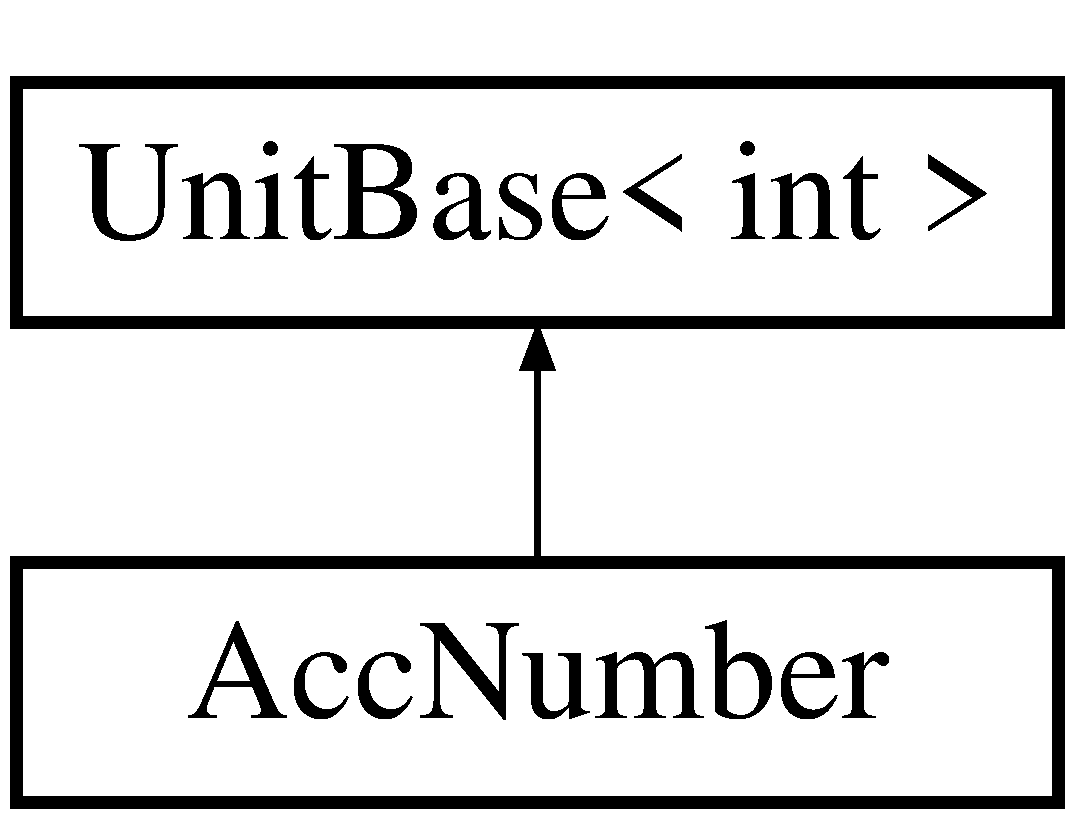
\includegraphics[height=2.000000cm]{classAccNumber}
\end{center}
\end{figure}
\subsection*{Public Member Functions}
\begin{DoxyCompactItemize}
\item 
\hypertarget{classAccNumber_a11a8a2ea0849a83365960758a5ff3362}{{\bfseries Acc\-Number} (int)  throw (invalid\-\_\-argument)}\label{classAccNumber_a11a8a2ea0849a83365960758a5ff3362}

\end{DoxyCompactItemize}
\subsection*{Additional Inherited Members}


\subsection{Detailed Description}
Define o número da conta de um Customer (Cliente). 

Este tipo básico tem a função de atribuir a cada conta um numero unico, identificando-\/a. 

The documentation for this class was generated from the following files\-:\begin{DoxyCompactItemize}
\item 
Base\-Unit.\-h\item 
Base\-Unit.\-cpp\end{DoxyCompactItemize}

\hypertarget{classMoney}{\section{Money Class Reference}
\label{classMoney}\index{Money@{Money}}
}


Define o limite da conta de um Customer (Cliente).  




{\ttfamily \#include $<$Base\-Unit.\-h$>$}

Inheritance diagram for Money\-:\begin{figure}[H]
\begin{center}
\leavevmode
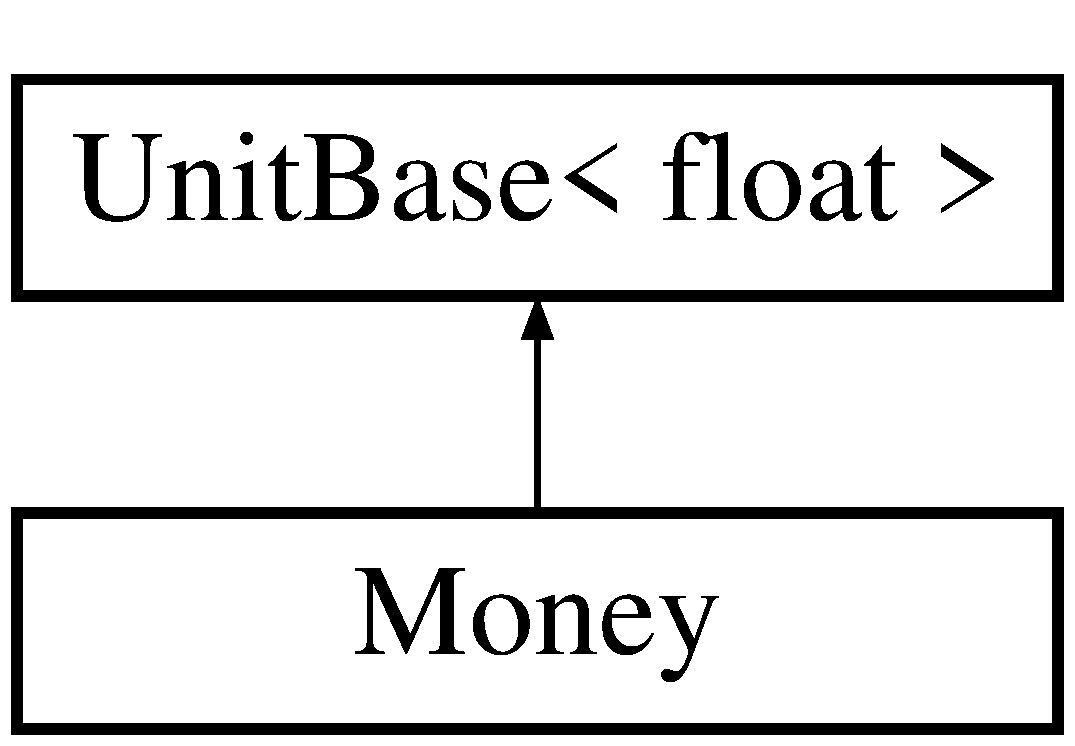
\includegraphics[height=2.000000cm]{classMoney}
\end{center}
\end{figure}
\subsection*{Public Member Functions}
\begin{DoxyCompactItemize}
\item 
\hypertarget{classMoney_a1b60c57dfd3140ad8c1ab4b831767ef0}{{\bfseries Money} (float)  throw (invalid\-\_\-argument)}\label{classMoney_a1b60c57dfd3140ad8c1ab4b831767ef0}

\end{DoxyCompactItemize}
\subsection*{Additional Inherited Members}


\subsection{Detailed Description}
Define o limite da conta de um Customer (Cliente). 

Atribui a cada conta um limite, limitando a utilização do crédito junto ao banco. 

The documentation for this class was generated from the following file\-:\begin{DoxyCompactItemize}
\item 
Base\-Unit.\-h\end{DoxyCompactItemize}

\hypertarget{classPayCode}{\section{Pay\-Code Class Reference}
\label{classPayCode}\index{Pay\-Code@{Pay\-Code}}
}


Define um número de identificação para cada pagamento.  




{\ttfamily \#include $<$Base\-Unit.\-h$>$}

Inheritance diagram for Pay\-Code\-:\begin{figure}[H]
\begin{center}
\leavevmode
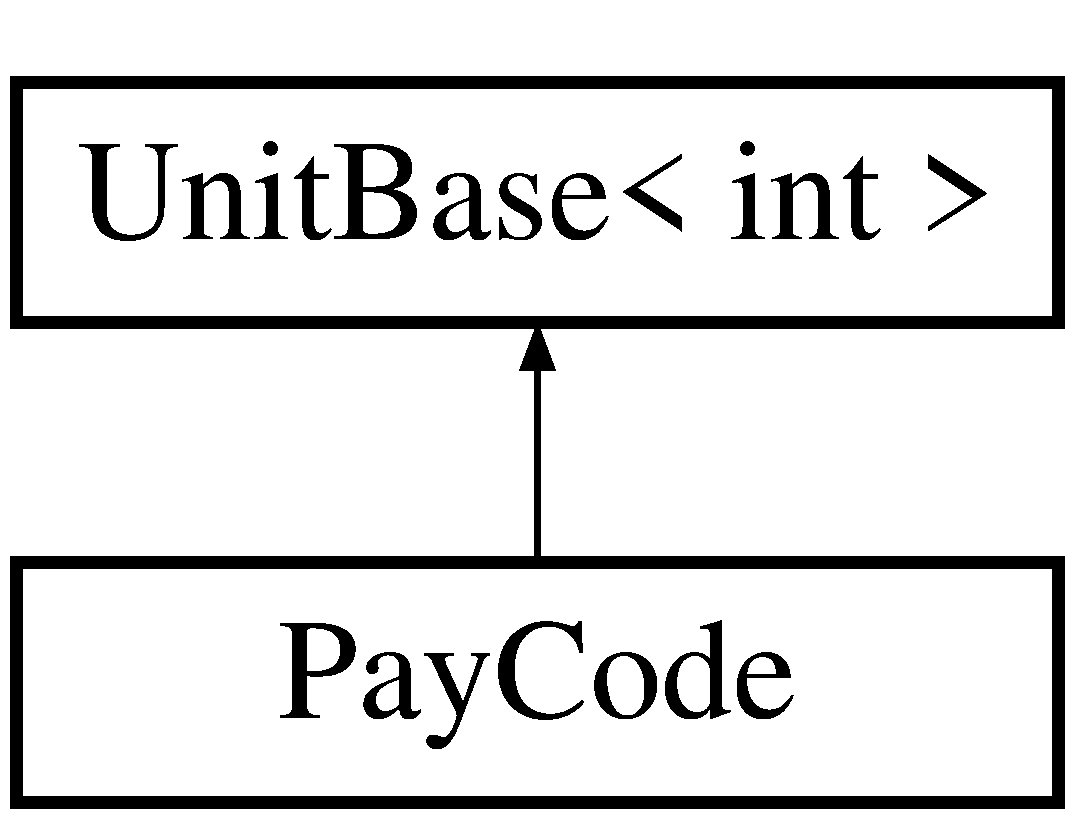
\includegraphics[height=2.000000cm]{classPayCode}
\end{center}
\end{figure}
\subsection*{Public Member Functions}
\begin{DoxyCompactItemize}
\item 
\hypertarget{classPayCode_aa867c5138d3d6858cfc7d87d08ef9599}{{\bfseries Pay\-Code} (int)  throw (invalid\-\_\-argument)}\label{classPayCode_aa867c5138d3d6858cfc7d87d08ef9599}

\end{DoxyCompactItemize}
\subsection*{Additional Inherited Members}


\subsection{Detailed Description}
Define um número de identificação para cada pagamento. 

Atribui a cada pagamento um código, de forma a identificá-\/lo. 

The documentation for this class was generated from the following files\-:\begin{DoxyCompactItemize}
\item 
Base\-Unit.\-h\item 
Base\-Unit.\-cpp\end{DoxyCompactItemize}

\hypertarget{classPayDay}{\section{Pay\-Day Class Reference}
\label{classPayDay}\index{Pay\-Day@{Pay\-Day}}
}


Define a data do pagamento.  




{\ttfamily \#include $<$Base\-Unit.\-h$>$}

Inheritance diagram for Pay\-Day\-:\begin{figure}[H]
\begin{center}
\leavevmode
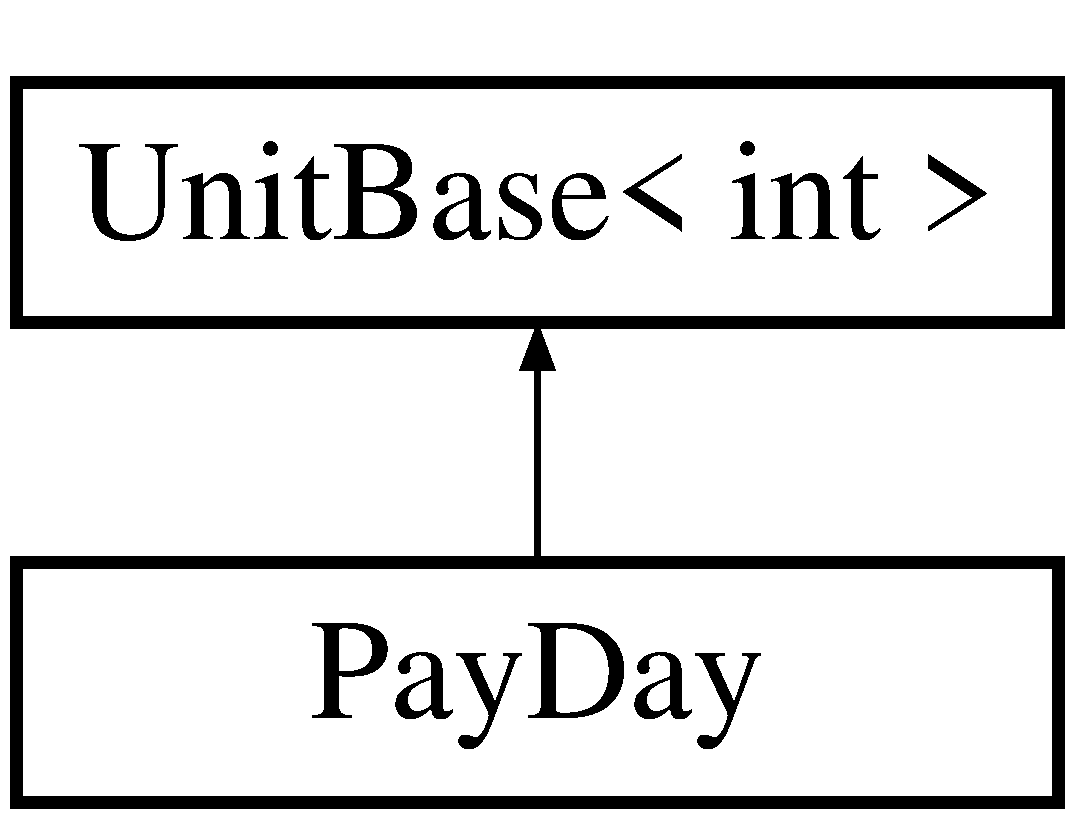
\includegraphics[height=2.000000cm]{classPayDay}
\end{center}
\end{figure}
\subsection*{Public Member Functions}
\begin{DoxyCompactItemize}
\item 
\hypertarget{classPayDay_a8b78191ec9a71a44086a2ca6a54a2303}{{\bfseries Pay\-Day} (int)  throw (invalid\-\_\-argument)}\label{classPayDay_a8b78191ec9a71a44086a2ca6a54a2303}

\item 
\hypertarget{classPayDay_a297ce892f49aa9f3a504d514f171ed1d}{int {\bfseries day} ()}\label{classPayDay_a297ce892f49aa9f3a504d514f171ed1d}

\item 
\hypertarget{classPayDay_ada65e8834c142a95cd35ca2b399fbcde}{int {\bfseries month} ()}\label{classPayDay_ada65e8834c142a95cd35ca2b399fbcde}

\item 
\hypertarget{classPayDay_a962960925f9e6eaaac0fef5eb96849ec}{int {\bfseries year} ()}\label{classPayDay_a962960925f9e6eaaac0fef5eb96849ec}

\end{DoxyCompactItemize}
\subsection*{Additional Inherited Members}


\subsection{Detailed Description}
Define a data do pagamento. 

Guarda a data de um pagamento. Dia, mês e ano devem ser acessados através dos atributos day, month, year. 

The documentation for this class was generated from the following file\-:\begin{DoxyCompactItemize}
\item 
Base\-Unit.\-h\end{DoxyCompactItemize}

\hypertarget{classPayValue}{\section{Pay\-Value Class Reference}
\label{classPayValue}\index{Pay\-Value@{Pay\-Value}}
}


Define o valor do pagamento.  




{\ttfamily \#include $<$Base\-Unit.\-h$>$}

Inheritance diagram for Pay\-Value\-:\begin{figure}[H]
\begin{center}
\leavevmode
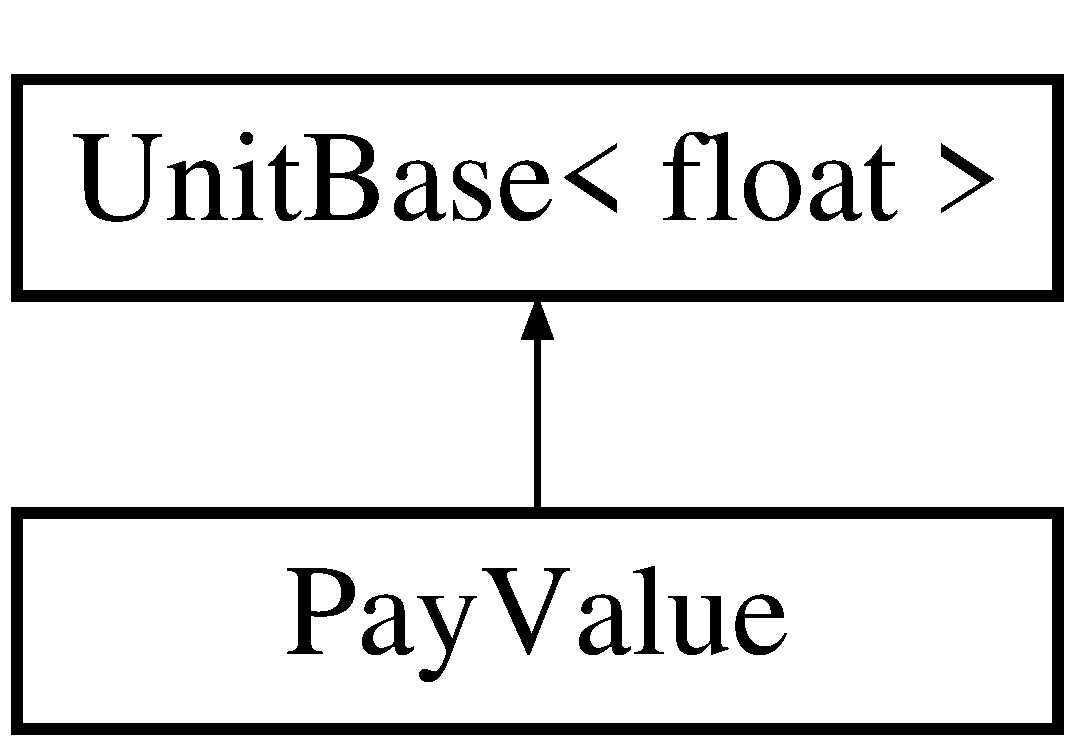
\includegraphics[height=2.000000cm]{classPayValue}
\end{center}
\end{figure}
\subsection*{Public Member Functions}
\begin{DoxyCompactItemize}
\item 
\hypertarget{classPayValue_a94fd7f5521beb8a47dbd34e6e0671a11}{{\bfseries Pay\-Value} (float)  throw (invalid\-\_\-argument)}\label{classPayValue_a94fd7f5521beb8a47dbd34e6e0671a11}

\end{DoxyCompactItemize}
\subsection*{Additional Inherited Members}


\subsection{Detailed Description}
Define o valor do pagamento. 

Recorda o valor de um pagamento. 

The documentation for this class was generated from the following files\-:\begin{DoxyCompactItemize}
\item 
Base\-Unit.\-h\item 
Base\-Unit.\-cpp\end{DoxyCompactItemize}

\hypertarget{classUnitBase}{\section{Unit\-Base$<$ base\-Type $>$ Class Template Reference}
\label{classUnitBase}\index{Unit\-Base$<$ base\-Type $>$@{Unit\-Base$<$ base\-Type $>$}}
}


A base de derivação de todas as classes de tipos básicos.  




{\ttfamily \#include $<$Base\-Unit.\-h$>$}

\subsection*{Public Member Functions}
\begin{DoxyCompactItemize}
\item 
\hypertarget{classUnitBase_af14e2453bc9870f0e04514799585e763}{void {\bfseries set\-Value} (const base\-Type \&value)  throw (invalid\-\_\-argument)}\label{classUnitBase_af14e2453bc9870f0e04514799585e763}

\item 
\hypertarget{classUnitBase_a620b2e9bda880c77d98a3c4cafb8443f}{base\-Type {\bfseries get\-Value} ()}\label{classUnitBase_a620b2e9bda880c77d98a3c4cafb8443f}

\end{DoxyCompactItemize}
\subsection*{Protected Attributes}
\begin{DoxyCompactItemize}
\item 
\hypertarget{classUnitBase_a1c1ad08b45f07a94e5cf71dee734436b}{base\-Type {\bfseries value}}\label{classUnitBase_a1c1ad08b45f07a94e5cf71dee734436b}

\end{DoxyCompactItemize}


\subsection{Detailed Description}
\subsubsection*{template$<$typename base\-Type$>$class Unit\-Base$<$ base\-Type $>$}

A base de derivação de todas as classes de tipos básicos. 

Suas diferentes instâncias servem de base para a construção de todos os outros tipos básicos. Seus métodos ser\-Value() e get\-Value() garantem o acesso ao seu parâmetro Value. 

The documentation for this class was generated from the following file\-:\begin{DoxyCompactItemize}
\item 
Base\-Unit.\-h\end{DoxyCompactItemize}

\hypertarget{classUsrId}{\section{Usr\-Id Class Reference}
\label{classUsrId}\index{Usr\-Id@{Usr\-Id}}
}


Define o I\-D de um Customer.  




{\ttfamily \#include $<$Base\-Unit.\-h$>$}

Inheritance diagram for Usr\-Id\-:\begin{figure}[H]
\begin{center}
\leavevmode
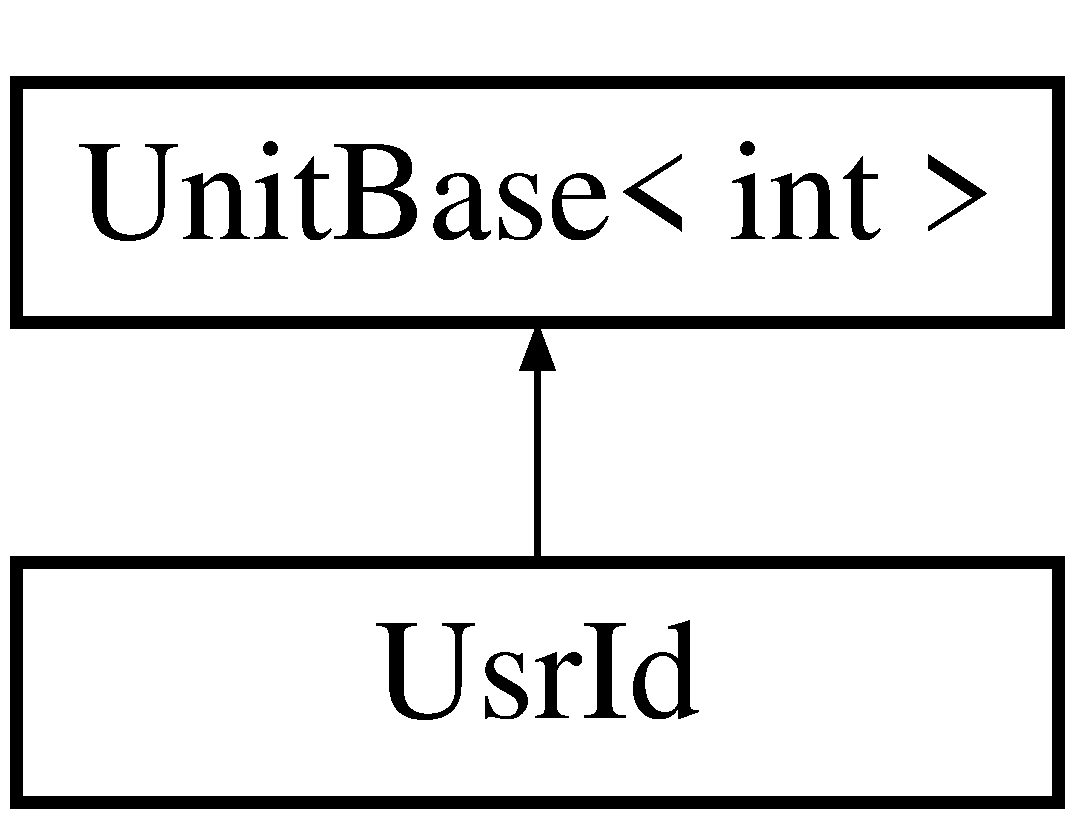
\includegraphics[height=2.000000cm]{classUsrId}
\end{center}
\end{figure}
\subsection*{Public Member Functions}
\begin{DoxyCompactItemize}
\item 
\hypertarget{classUsrId_a90f49e923fb187c5330f71a75cd643a2}{{\bfseries Id} ()}\label{classUsrId_a90f49e923fb187c5330f71a75cd643a2}

\item 
\hypertarget{classUsrId_a492418ee700c6a34d1dda28054b369b0}{{\bfseries Id} (int)  throw (invalid\-\_\-argument)}\label{classUsrId_a492418ee700c6a34d1dda28054b369b0}

\end{DoxyCompactItemize}
\subsection*{Additional Inherited Members}


\subsection{Detailed Description}
Define o I\-D de um Customer. 

Tem a função de identificar de forma única um Customer, independentemente do seu tipo de conta. 

The documentation for this class was generated from the following files\-:\begin{DoxyCompactItemize}
\item 
Base\-Unit.\-h\item 
Base\-Unit.\-c\end{DoxyCompactItemize}

\hypertarget{classUsrMatric}{\section{Usr\-Matric Class Reference}
\label{classUsrMatric}\index{Usr\-Matric@{Usr\-Matric}}
}


Define a matrícula de um Manager.  




{\ttfamily \#include $<$Base\-Unit.\-h$>$}

Inheritance diagram for Usr\-Matric\-:\begin{figure}[H]
\begin{center}
\leavevmode
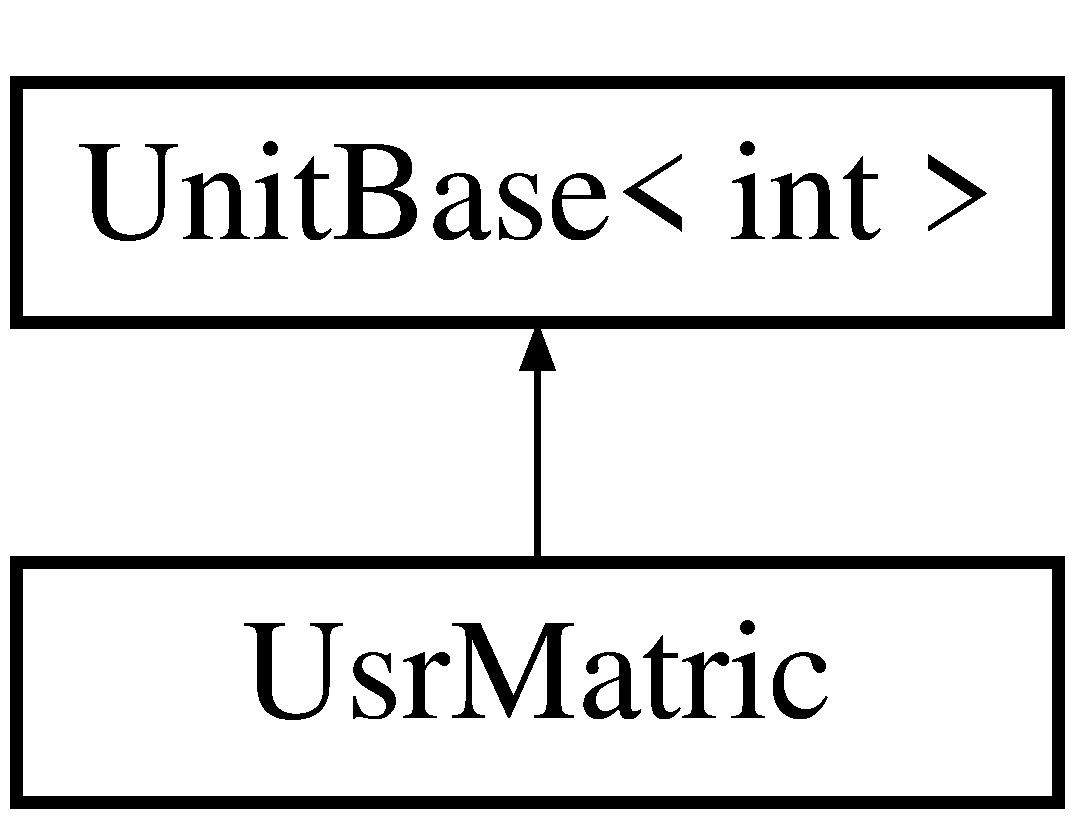
\includegraphics[height=2.000000cm]{classUsrMatric}
\end{center}
\end{figure}
\subsection*{Public Member Functions}
\begin{DoxyCompactItemize}
\item 
\hypertarget{classUsrMatric_a62732ab82c25990f4e37ad7575760630}{{\bfseries Matric} ()}\label{classUsrMatric_a62732ab82c25990f4e37ad7575760630}

\item 
\hypertarget{classUsrMatric_a986f012bd822779ed3a256dddfd26581}{{\bfseries Matric} (int)  throw (invalid\-\_\-argument)}\label{classUsrMatric_a986f012bd822779ed3a256dddfd26581}

\end{DoxyCompactItemize}
\subsection*{Additional Inherited Members}


\subsection{Detailed Description}
Define a matrícula de um Manager. 

Tem a função de identificar de forma única um Manager, seja ele Administrador ou Gerente. 

The documentation for this class was generated from the following files\-:\begin{DoxyCompactItemize}
\item 
Base\-Unit.\-h\item 
Base\-Unit.\-cpp\end{DoxyCompactItemize}

\hypertarget{classUsrName}{\section{Usr\-Name Class Reference}
\label{classUsrName}\index{Usr\-Name@{Usr\-Name}}
}


Define o nome de um \hyperlink{classUser}{User} (Customer ou Manager).  




{\ttfamily \#include $<$Base\-Unit.\-h$>$}

Inheritance diagram for Usr\-Name\-:\begin{figure}[H]
\begin{center}
\leavevmode
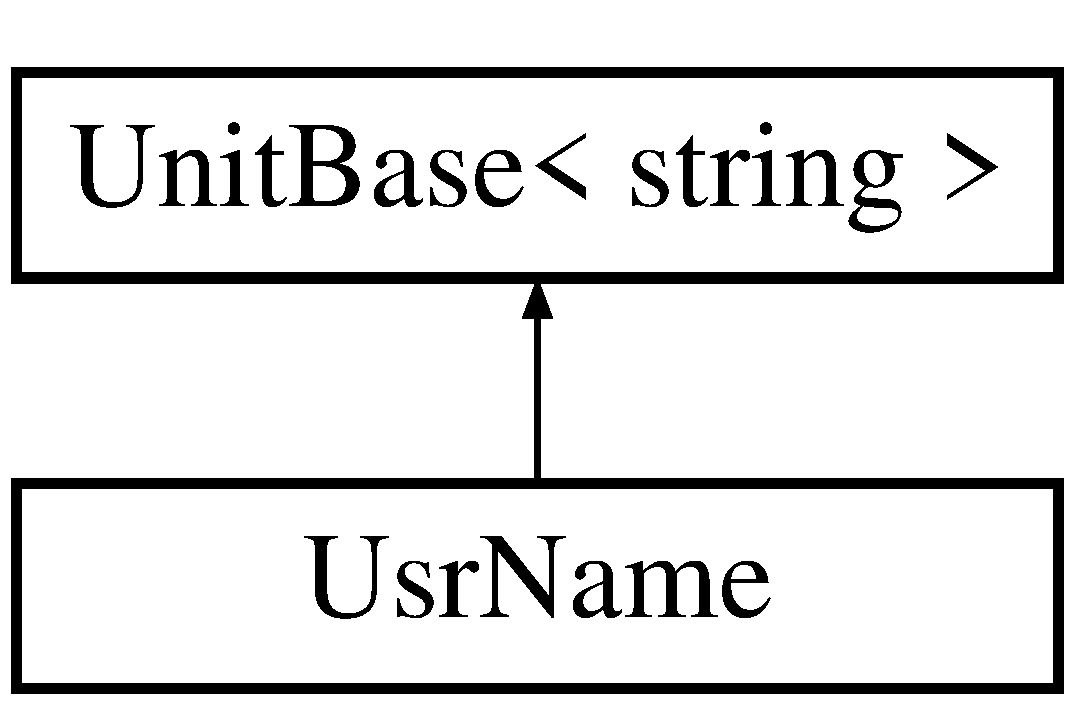
\includegraphics[height=2.000000cm]{classUsrName}
\end{center}
\end{figure}
\subsection*{Public Member Functions}
\begin{DoxyCompactItemize}
\item 
\hypertarget{classUsrName_a1b08302bcdce4624efc4283717bf0156}{{\bfseries Name} ()}\label{classUsrName_a1b08302bcdce4624efc4283717bf0156}

\item 
\hypertarget{classUsrName_aa28a3613ce9157f86f56cd038d288df2}{{\bfseries Name} (string)  throw (invalid\-\_\-argument)}\label{classUsrName_aa28a3613ce9157f86f56cd038d288df2}

\end{DoxyCompactItemize}
\subsection*{Additional Inherited Members}


\subsection{Detailed Description}
Define o nome de um \hyperlink{classUser}{User} (Customer ou Manager). 

Este tipo serve para regular o login de usuários em geral. 

The documentation for this class was generated from the following file\-:\begin{DoxyCompactItemize}
\item 
Base\-Unit.\-h\end{DoxyCompactItemize}

\hypertarget{classUsrPassword}{\section{Usr\-Password Class Reference}
\label{classUsrPassword}\index{Usr\-Password@{Usr\-Password}}
}


Define a senha de um User (Customer ou Manager).  




{\ttfamily \#include $<$Base\-Unit.\-h$>$}

Inheritance diagram for Usr\-Password\-:\begin{figure}[H]
\begin{center}
\leavevmode
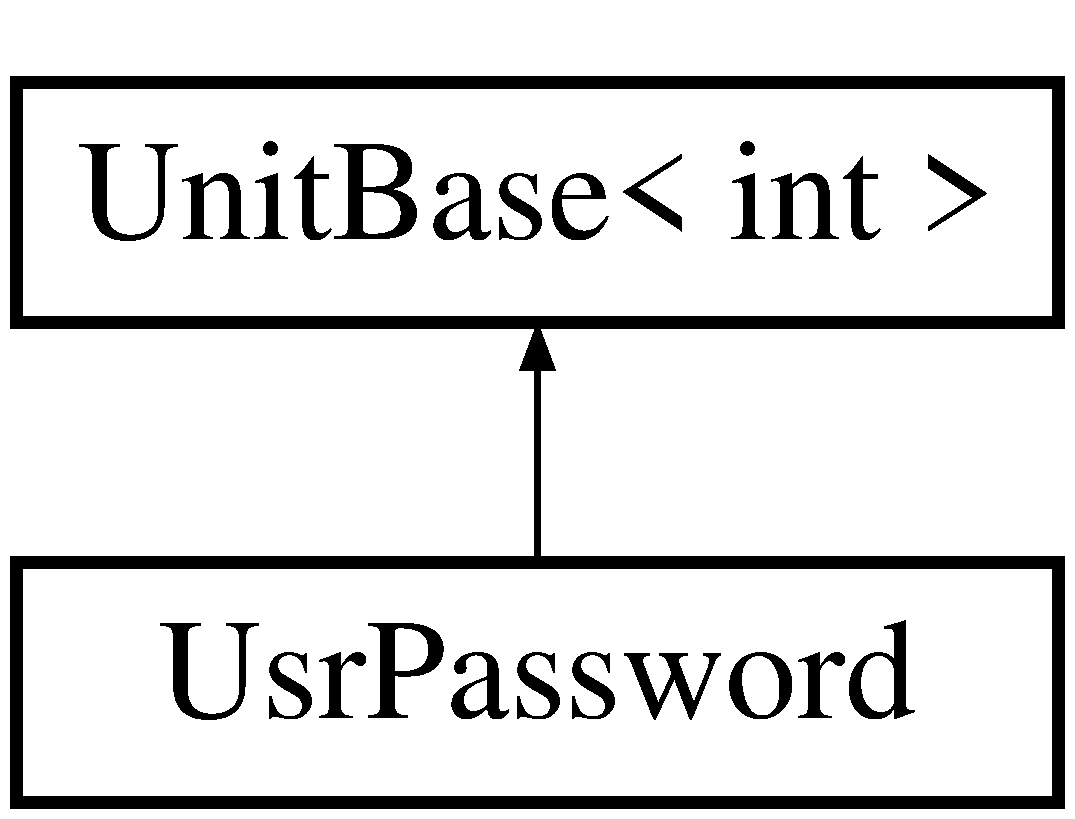
\includegraphics[height=2.000000cm]{classUsrPassword}
\end{center}
\end{figure}
\subsection*{Public Member Functions}
\begin{DoxyCompactItemize}
\item 
\hypertarget{classUsrPassword_ad08a7c4a7e940186d4d23a5347ea7080}{{\bfseries Password} ()}\label{classUsrPassword_ad08a7c4a7e940186d4d23a5347ea7080}

\item 
\hypertarget{classUsrPassword_a42ff4b71c0c413ae5db79ea2697cc7a6}{{\bfseries Password} (int)  throw (invalid\-\_\-argument)}\label{classUsrPassword_a42ff4b71c0c413ae5db79ea2697cc7a6}

\end{DoxyCompactItemize}
\subsection*{Additional Inherited Members}


\subsection{Detailed Description}
Define a senha de um User (Customer ou Manager). 

Este tipo básico tem a função de controlar o login de usuários em geral. 

The documentation for this class was generated from the following file\-:\begin{DoxyCompactItemize}
\item 
Base\-Unit.\-h\end{DoxyCompactItemize}

\hypertarget{classUsrType}{\section{Usr\-Type Class Reference}
\label{classUsrType}\index{Usr\-Type@{Usr\-Type}}
}


Codifica tipos de conta.  




{\ttfamily \#include $<$Base\-Unit.\-h$>$}

Inheritance diagram for Usr\-Type\-:\begin{figure}[H]
\begin{center}
\leavevmode
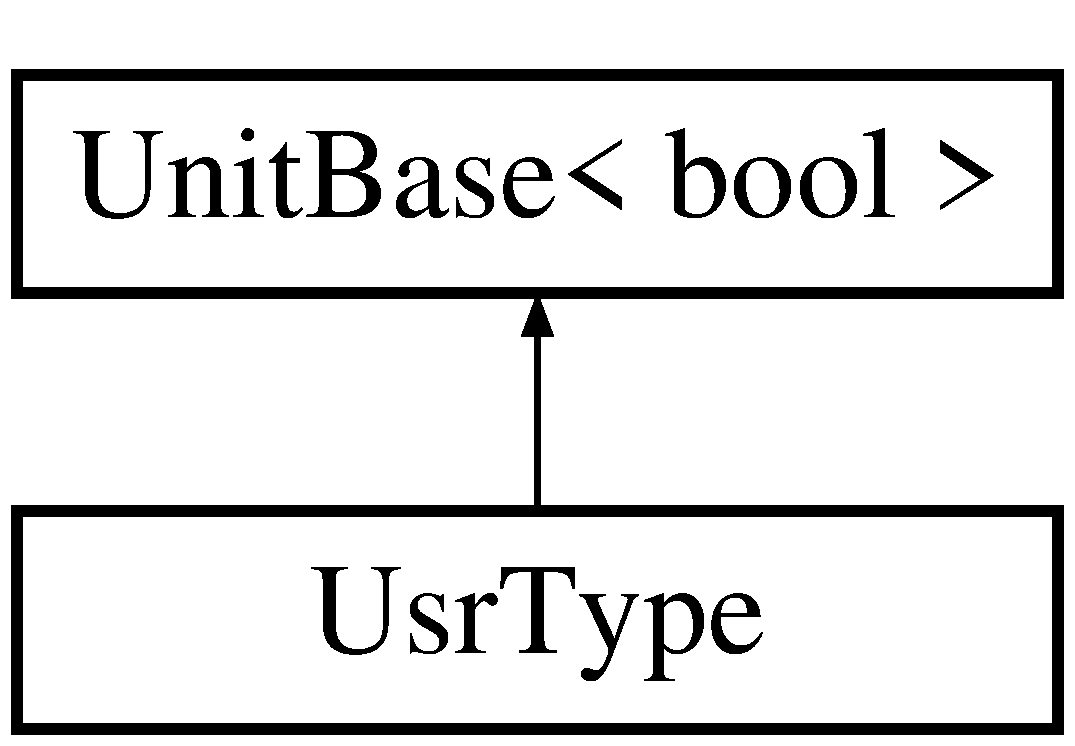
\includegraphics[height=2.000000cm]{classUsrType}
\end{center}
\end{figure}
\subsection*{Public Member Functions}
\begin{DoxyCompactItemize}
\item 
\hypertarget{classUsrType_a551a40c57ccc7dec21a42e539ff5899c}{{\bfseries G\-Type} ()}\label{classUsrType_a551a40c57ccc7dec21a42e539ff5899c}

\item 
\hypertarget{classUsrType_a4b88730c90e740fa4e9ca4d247ee8616}{{\bfseries G\-Type} (bool)}\label{classUsrType_a4b88730c90e740fa4e9ca4d247ee8616}

\end{DoxyCompactItemize}
\subsection*{Additional Inherited Members}


\subsection{Detailed Description}
Codifica tipos de conta. 

Possui duas utilizações\-: Acc\-Type\-: Codifica tipos de conta (Normal / Especial) Man\-Type\-: Codifica tipos de manager (Gerente / Administrador) 

The documentation for this class was generated from the following files\-:\begin{DoxyCompactItemize}
\item 
Base\-Unit.\-h\item 
Base\-Unit.\-cpp\end{DoxyCompactItemize}

\addcontentsline{toc}{part}{Index}
\printindex
\end{document}
